%%%%%%%%%%%%%%%%%%%%%%%%%%%%%%%%%%%%%%%%%
%
% CMPT 424
% Fall 2022
% Lab 5
%
%%%%%%%%%%%%%%%%%%%%%%%%%%%%%%%%%%%%%%%%%

%%%%%%%%%%%%%%%%%%%%%%%%%%%%%%%%%%%%%%%%%
% Short Sectioned Assignment
% LaTeX Template
% Version 1.0 (5/5/12)
%
% This template has been downloaded from: http://www.LaTeXTemplates.com
% Original author: % Frits Wenneker (http://www.howtotex.com)
% License: CC BY-NC-SA 3.0 (http://creativecommons.org/licenses/by-nc-sa/3.0/)
% Modified by Alan G. Labouseur  - alan@labouseur.com
%
%%%%%%%%%%%%%%%%%%%%%%%%%%%%%%%%%%%%%%%%%

%----------------------------------------------------------------------------------------
%	PACKAGES AND OTHER DOCUMENT CONFIGURATIONS
%----------------------------------------------------------------------------------------

\documentclass[letterpaper, 10pt,DIV=13]{scrartcl} 

\usepackage[T1]{fontenc} % Use 8-bit encoding that has 256 glyphs
\usepackage[english]{babel} % English language/hyphenation
\usepackage{amsmath,amsfonts,amsthm,xfrac} % Math packages
\usepackage{sectsty} % Allows customizing section commands
\usepackage{graphicx}
\usepackage[lined,linesnumbered,commentsnumbered]{algorithm2e}
\usepackage{listings}
\usepackage{parskip}
\usepackage{lastpage}

\allsectionsfont{\normalfont\scshape} % Make all section titles in default font and small caps.

\usepackage{fancyhdr} % Custom headers and footers
\pagestyle{fancyplain} % Makes all pages in the document conform to the custom headers and footers

\fancyhead{} % No page header - if you want one, create it in the same way as the footers below
\fancyfoot[L]{} % Empty left footer
\fancyfoot[C]{} % Empty center footer
\fancyfoot[R]{page \thepage\ of \pageref{LastPage}} % Page numbering for right footer

\renewcommand{\headrulewidth}{0pt} % Remove header underlines
\renewcommand{\footrulewidth}{0pt} % Remove footer underlines
\setlength{\headheight}{13.6pt} % Customize the height of the header

\numberwithin{equation}{section} % Number equations within sections (i.e. 1.1, 1.2, 2.1, 2.2 instead of 1, 2, 3, 4)
\numberwithin{figure}{section} % Number figures within sections (i.e. 1.1, 1.2, 2.1, 2.2 instead of 1, 2, 3, 4)
\numberwithin{table}{section} % Number tables within sections (i.e. 1.1, 1.2, 2.1, 2.2 instead of 1, 2, 3, 4)

\setlength\parindent{0pt} % Removes all indentation from paragraphs.

\binoppenalty=3000
\relpenalty=3000

%----------------------------------------------------------------------------------------
%	TITLE SECTION
%----------------------------------------------------------------------------------------

\newcommand{\horrule}[1]{\rule{\linewidth}{#1}} % Create horizontal rule command with 1 argument of height

\title{	
   \normalfont \normalsize 
   \textsc{CMPT 424 - Fall 2022 - Dr. Labouseur} \\[10pt] % Header stuff.
   \horrule{0.5pt} \\[0.25cm] 	% Top horizontal rule
   \huge Lab 5  \\     	    % Assignment title
   \horrule{0.5pt} \\[0.25cm] 	% Bottom horizontal rule
}

\author{Josh Seligman \\ \normalsize joshua.seligman1@marist.edu}

\date{\normalsize\today} 	% Today's date.

\begin{document}
\maketitle % Print the title

% Question 1
\section{Question 1}
\subsection{Part A}
\textit{Draw your Gantt charts that illustrate the execution of these processes using the fillowing scheduling algorithms: FCFS, SJF, nonpreemprive priority, and RR (quantum = 1).}

See Figure \ref{fig:ganttCharts}

\subsection{Part B}
\textit{What is the turnaround time of each process for each of the scheduling algorithms in part a?}

FCFS: P1 = 10, P2 = 11, P3 = 13, P4 = 14, P5 = 19 \\
SJF: P1 = 19, P2 = 1, P4 = 2, P3 = 4, P5 = 9 \\
NP Priority: P1 = 16, P2 = 1, P3 = 18, P4 = 19, P5 = 6 \\
RR: P1 = 19, P2 = 2, P3 = 7, P4 = 4, P5 = 14


\subsection{Part C}
\textit{What is the waiting time of each process for each of these scheduling algorithms?}

FCFS: P1 = 0, P2 = 10, P3 = 11, P4 = 13, P5 = 14 \\
SJF: P1 = 9, P2 = 0, P3 = 2, P4 = 1, P5 = 4 \\
NP Priority: P1 = 6, P2 = 0, P3 = 16, P4 = 18, P5 = 1 \\
RR: P1 = 4 + 2 + 1 + 1 + 1 = 9, P2 = 1, P3 = 2 + 3 = 5, P4 = 3, P5 = 4 + 2 + 1 + 1 + 1 = 9


\subsection{Part D}
\textit{Which of the algorithms results in the minimum average wating time (over all processes)?}

FCFS = (0 + 10 + 11 + 13 + 14) / 5 = 9.6 \\
SJF = (9 + 0 + 2 + 1 + 4) / 5= 3.2 \\
NP Priority: (6 + 0 + 16 + 18 + 1) / 5 = 8.2 \\
RR: (9 + 1 + 5 + 3 + 9) / 5 = 5.4

SJF has the smallest average waiting time.


\begin{figure}[ht] 
   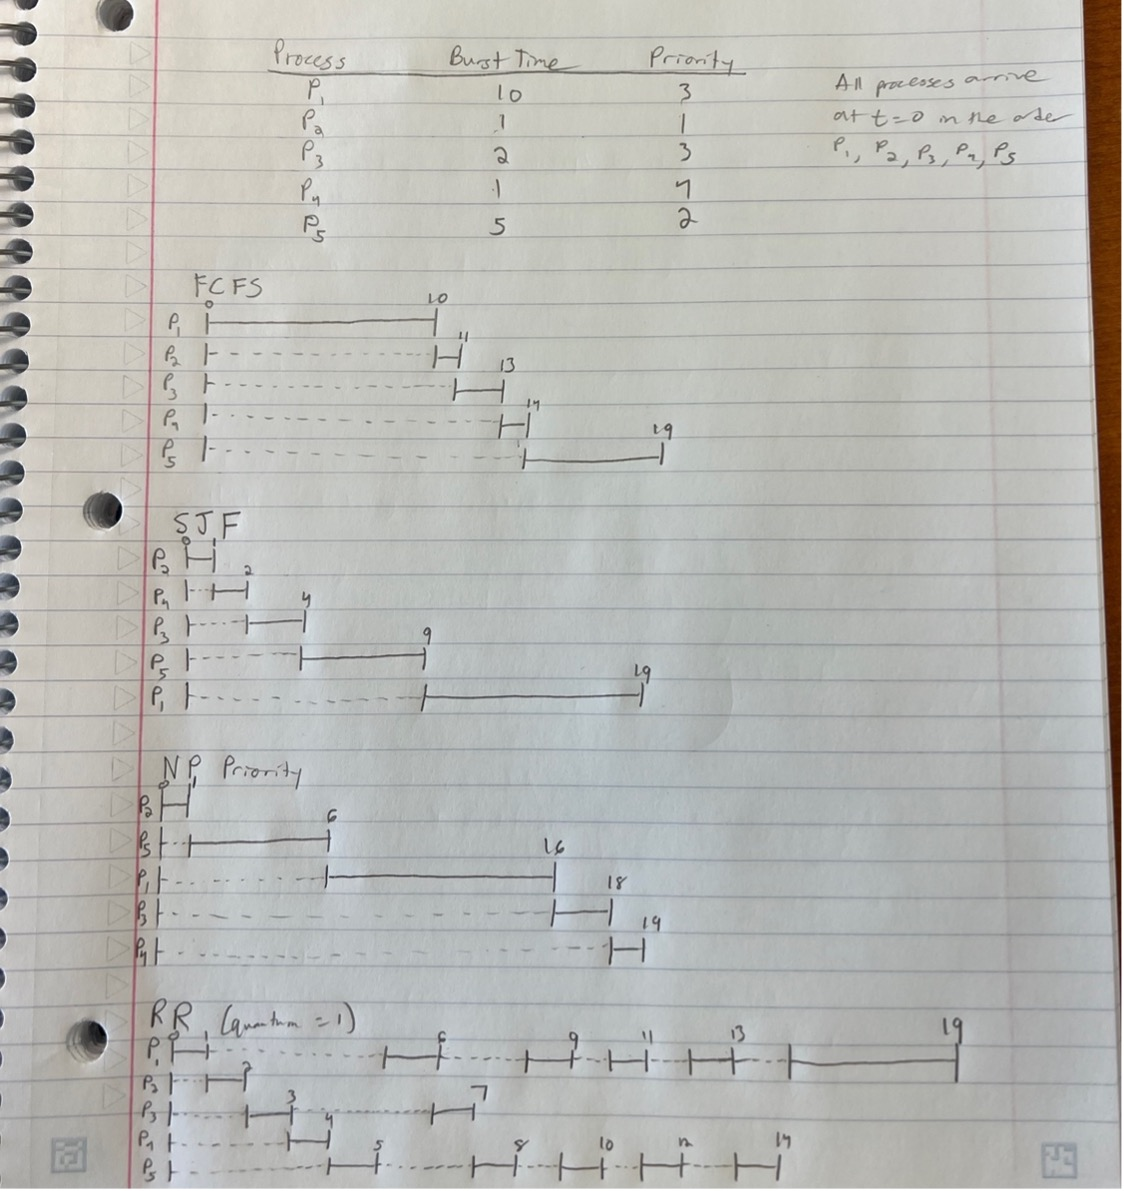
\includegraphics[height=12cm]{ganttCharts.jpg}
   \caption{The Gantt charts for each of the algorithms listed in part A.}
   \label{fig:ganttCharts}
\end{figure}

\end{document}
